\documentclass[12pt,a4paper]{article}
\usepackage{graphicx}
\usepackage{amsmath}
\usepackage{float}
\usepackage{hyperref}
\usepackage[top=0.3in]{geometry}


\title{Lab Report7}
\author{Arnav Yadnopavit EE24BTECH11007\\Prajwal EE24BTECH11051}
\date{\today}
\begin{document}
\maketitle
\section{Objective}
To design a Mod-7 Asynchronous Counter using JK Flip-Flops (JK FFs) and demonstrate its
performance using a CRO (Cathode Ray Oscilloscope) with a clock from an Arduino
\section{Components Required}
\begin{itemize}
    \item IC 7476 (Dual JK Flip-Flop)
    \item IC 7410 (Triple 3-input NAND Gate)
    \item Arduino UNO(for clock signal)
    \item 7-segment Anode dispaly to show count
    \item 7447 IC (7-segement display decoder)
    \item 220$\Omega$ Resistor
\end{itemize}
\section{Circuit}
\begin{table}[H]
    \centering
    \renewcommand{\arraystretch}{1.2}
    \begin{tabular}{|c|c|c|}
        \hline
        \textbf{Component} & \textbf{Pin} & \textbf{Connection} \\
        \hline
        \multicolumn{3}{|c|}{\textbf{Arduino Connections}} \\
        \hline
        Arduino & Pin 13 & Clock Input to First 7476 Flip-Flop \\
        \hline
        \multicolumn{3}{|c|}{\textbf{7476 (First Flip-Flop - Q1)}} \\
        \hline
        7476 (IC1) & VCC (Pin 16) & +5V \\
        7476 (IC1) & GND (Pin 8) & 0V (Ground) \\
        7476 (IC1) & J1, K1 & +5V (HIGH) \\
        7476 (IC1) & CLK1 & Arduino Pin 13 (Clock) \\
        7476 (IC1) & Q1 (Pin 15) & Clock for Second Flip-Flop \\
        7476 (IC1) & PRE1, CLR1 & +5V (HIGH) \\
        7476 (IC1) & CLR1 & Input from 7410 NAND Gate\\
        \hline
        \multicolumn{3}{|c|}{\textbf{7476 (Second Flip-Flop - Q2)}} \\
        \hline
        7476 (IC2) & J2, K2 & +5V (HIGH) \\
        7476 (IC2) & CLK2 & Q0 Output from First Flip-Flop \\
        7476 (IC2) & Q2 (Pin 15) & Input to 7410 NAND Gate \\
        7476 (IC2) & PRE2 & +5V (HIGH) \\
        7476 (IC2) & CLR2 & Input from 7410 NAND Gate\\
        \hline
        \multicolumn{3}{|c|}{\textbf{7476 (Second Flip-Flop - Q3)}} \\
        \hline
        7476 (IC3) & J3, K3 & +5V (HIGH) \\
        7476 (IC3) & CLK2 & Q1 Output from First Flip-Flop \\
        7476 (IC3) & Q3 (Pin 15) & Input to 7410 NAND Gate \\
        7476 (IC3) & PRE3 & +5V (HIGH) \\
        7476 (IC3) & CLR3 & Input from 7410 NAND Gate\\
        \hline
        \multicolumn{3}{|c|}{\textbf{7410 (NAND Gate for Reset)}} \\
        \hline
        7410 (IC3) & Input 1 & Q0 from 7476 \\
        7410 (IC3) & Input 2 & Q1 from 7476 \\
        7410 (IC3) & Input 3 & Q2 from 7476 \\
        7410 (IC3) & Output & CLR of Both 7476 Flip-Flops \\
        \hline
        \multicolumn{3}{|c|}{\textbf{7447 (BCD to 7-Segment Decoder)}} \\
        \hline
        7447 (IC4) & A (Pin 7) & Q0 from Flip-Flop \\
        7447 (IC4) & B (Pin 1) & Q1 from Flip-Flop \\
        7447 (IC4) & C (Pin 2) & Q2 from Flip-Flop \\
        7447 (IC4) & D (Pin 6) & GND (Always 0 for MOD-7 Counter) \\
        7447 (IC4) & Outputs (a-g) & Corresponding Pins of 7-Segment Display \\
        7447 (IC4) & VCC (Pin 16) & +5V \\
        7447 (IC4) & GND (Pin 8) & 0V (Ground) \\
        \hline
        \multicolumn{3}{|c|}{\textbf{7-Segment Display}} \\
        \hline
        7-Segment & a-g & Corresponding Pins from 7447 \\
        7-Segment & Common Anode & +5V via 220$\Omega$ Resistor \\
        \hline
    \end{tabular}
    \caption{Connections for Mod-7 Asynchronous Counter with Display}
    \label{tab:circuit}
\end{table}
\begin{figure}[H]
    \centering
    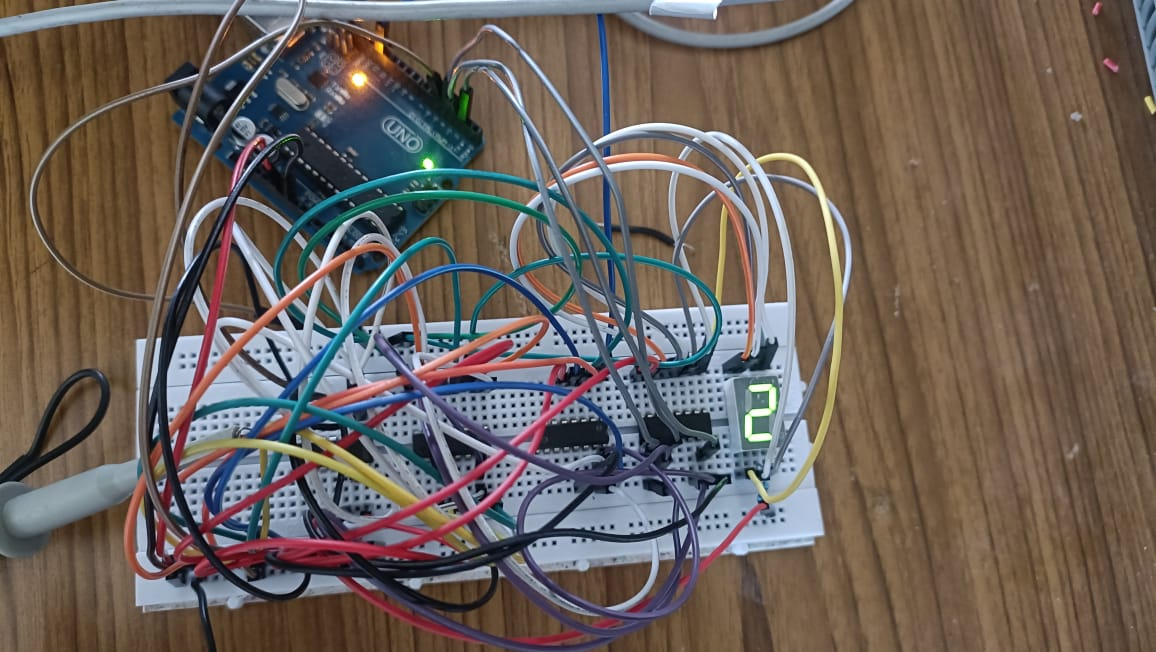
\includegraphics[width=0.7\textwidth]{figs/Circuit.jpeg} % Add your image file
    \caption{Circuit Diagram of Mod-7 Counter}
\end{figure}

\section{Truth Table}
\begin{table}[H]
    \centering
    \renewcommand{\arraystretch}{1.2}
    \begin{tabular}{|c|c|c|c|}
        \hline
        \textbf{J} & \textbf{K} & \textbf{Q (Previous State)} & \textbf{Q (Next State)} \\
        \hline
        0 & 0 & Q & Q (No Change) \\
        0 & 1 & Q & 0 (Reset) \\
        1 & 0 & Q & 1 (Set) \\
        1 & 1 & Q & $\overline{Q}$ (Toggle) \\
        \hline
    \end{tabular}
    \caption{Truth Table of JK Flip-Flop}
    \label{tab:jk_flipflop}
\end{table}

\begin{table}[H]
    \centering
    \begin{tabular}{|c|c|c|c|}
        \hline
        Clock Cycle & Q2 & Q1 & Q0 \\
        \hline
        0 & 0 & 0 & 0 \\
        1 & 0 & 0 & 1 \\
        2 & 0 & 1 & 0 \\
        3 & 0 & 1 & 1 \\
        4 & 1 & 0 & 0 \\
        5 & 1 & 0 & 1 \\
        6 & 1 & 1 & 0 \\
        7 & 0 & 0 & 0 (Reset) \\
        \hline
    \end{tabular}
    \caption{Truth Table for Mod-7 Counter}
    \label{tab:truth_table}
\end{table}

\section{Observations and Results}
\begin{figure}[H]
    \centering
    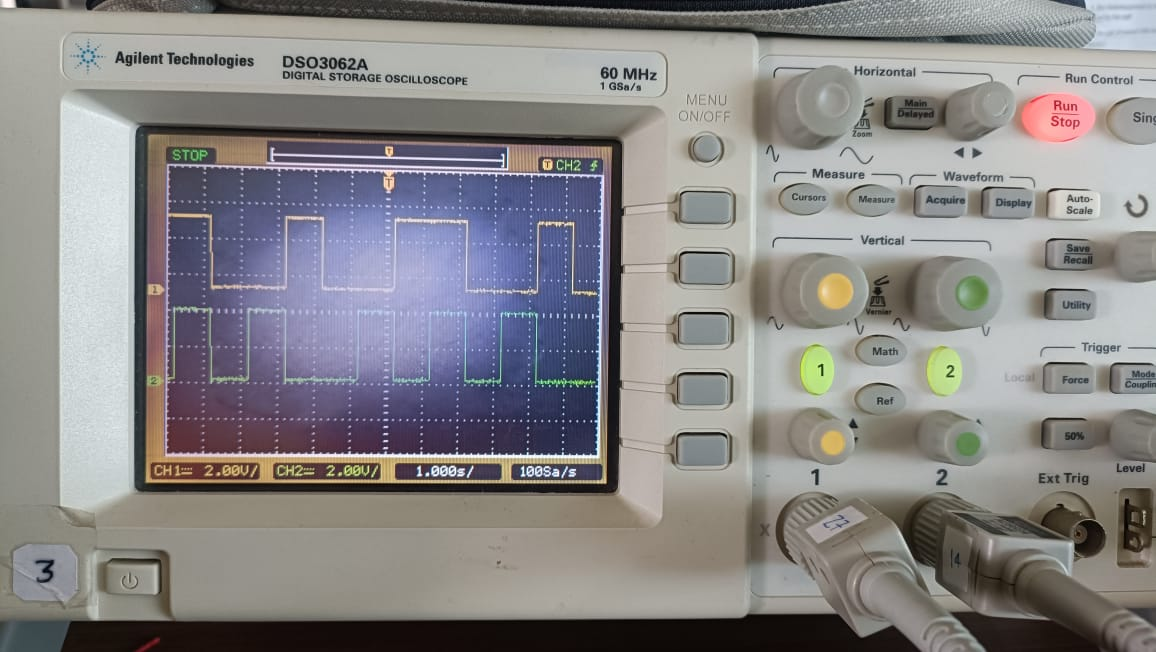
\includegraphics[width=0.7\textwidth]{figs/Q0Q1.jpeg} 
    \caption{Channel1-Q2,Channel2-Q1}
\end{figure}
\begin{figure}[H]
    \centering
    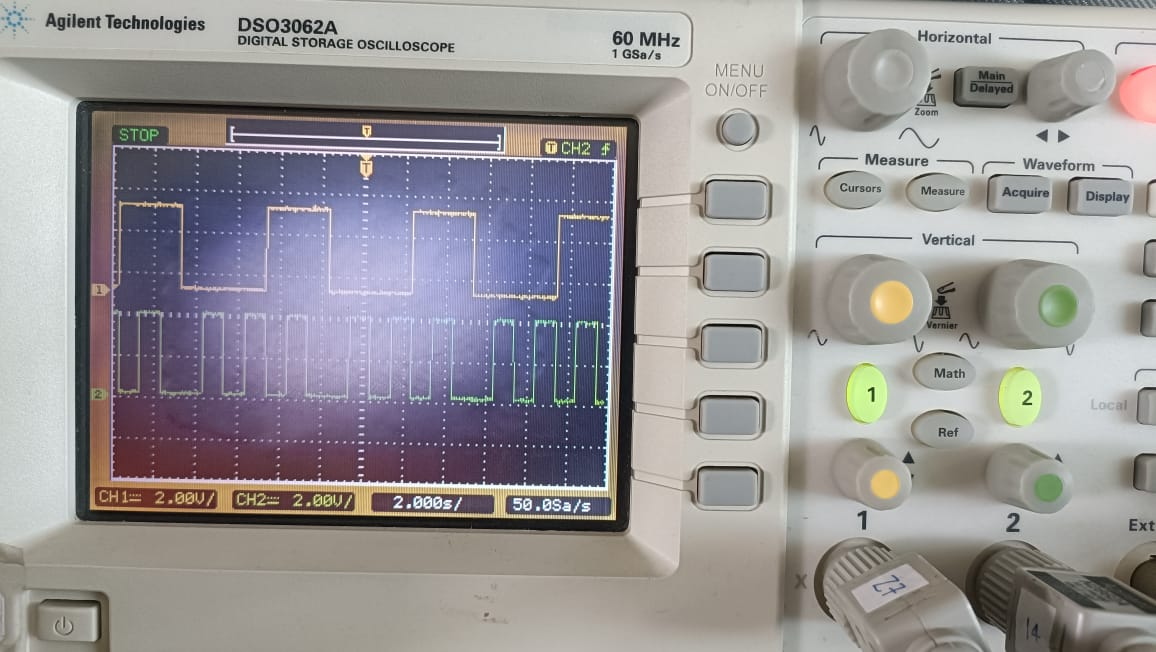
\includegraphics[width=0.7\textwidth]{figs/Q0Q2.jpeg} 
    \caption{Channel1-Q3,Channel2-Q1}
\end{figure}
\begin{figure}[H]
    \centering
    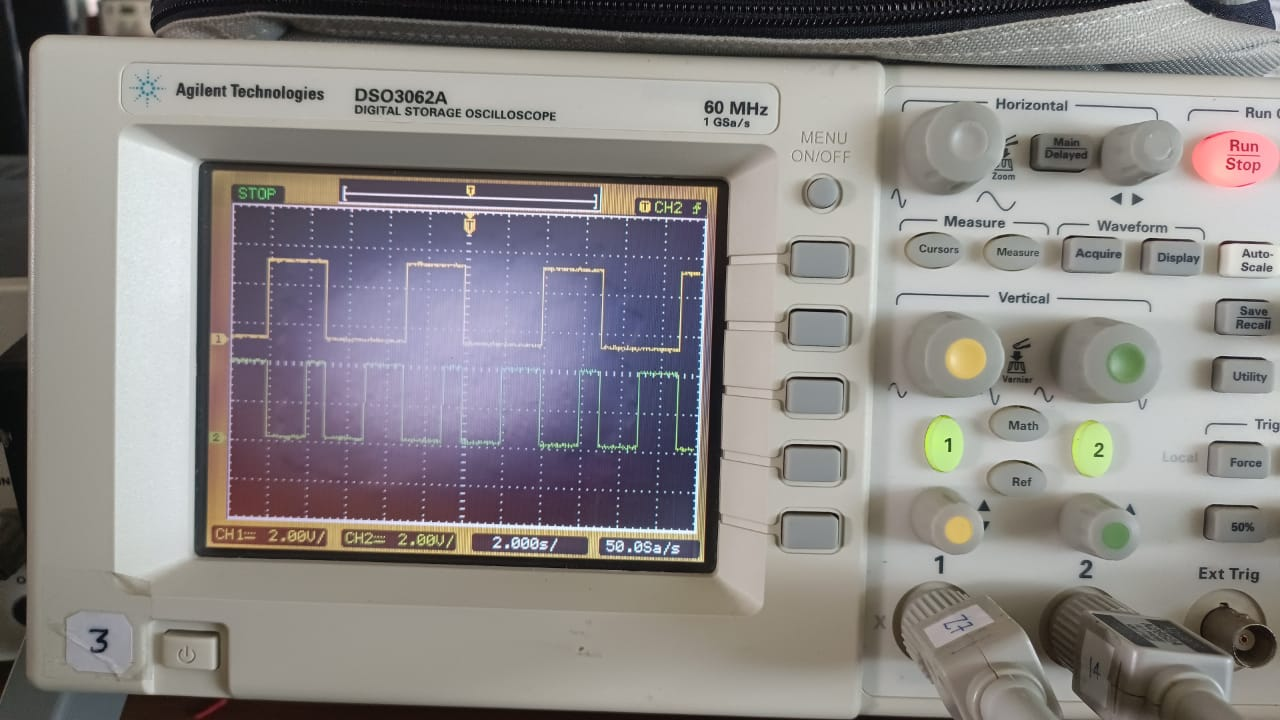
\includegraphics[width=0.7\textwidth]{figs/Q1Q2.jpeg} 
    \caption{Channel1-Q3,Channel2-Q2}
\end{figure}
\begin{figure}[H]
    \centering
    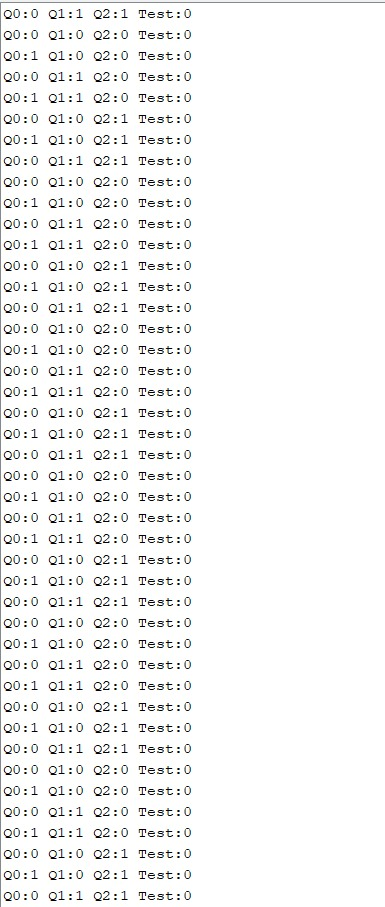
\includegraphics[width=0.7\textwidth]{figs/SerialMonitor.jpeg} 
    \caption{ArduinoSerialMonitor}
\end{figure}
\begin{figure}[H]
    \centering
    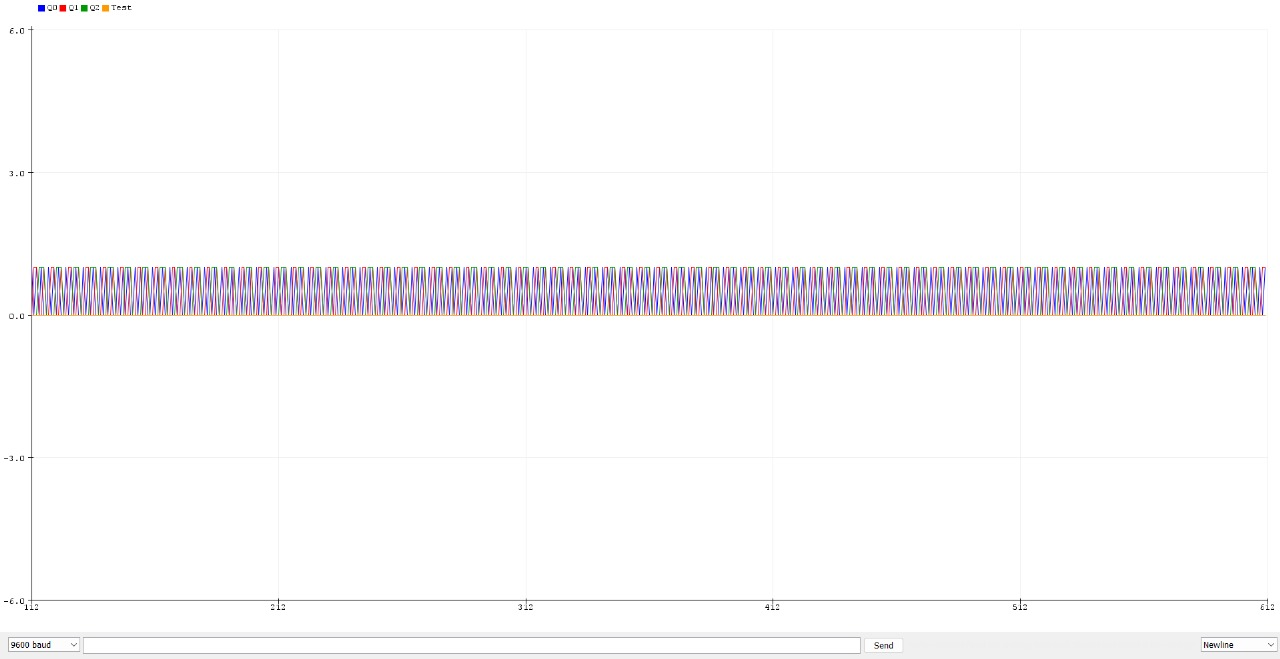
\includegraphics[width=0.7\textwidth]{figs/SerialPlotter.jpeg} 
    \caption{ArduinoSerialPlotter}
\end{figure}
\begin{itemize}
    \item The counter correctly cycles through states 0 to 6 before resetting.
    \item The clock signal from Arduino successfully triggered the JK flip-flops.
    \item The video of the counter is in the github repository.
\end{itemize}
To check the codes, video etc. refer \url{https://github.com/ArnavYadnopavit/ElectricalLabEE1200/tree/main/LabReport7}\\

\centering
Thank You
\end{document}

